% RECOMMENDED %%%%%%%%%%%%%%%%%%%%%%%%%%%%%%%%%%%%%%%%%%%%%%%%%%%
\documentclass[graybox,vecarrow]{styles/svmult}

% choose options for [] as required from the list
% in the Reference Guide

\usepackage{mathptmx}       % selects Times Roman as basic font
\usepackage{helvet}         % selects Helvetica as sans-serif font
\usepackage{courier}        % selects Courier as typewriter font
%\usepackage{type1cm}        % activate if the above 3 fonts are
                            % not available on your system

\usepackage{makeidx}         % allows index generation
\usepackage{graphicx}        % standard LaTeX graphics tool
                             % when including figure files
\usepackage{multicol}        % used for the two-column index
\usepackage[bottom]{footmisc}% places footnotes at page bottom

% see the list of further useful packages
% in the Reference Guide

\makeindex             % used for the subject index
                       % please use the style svind.ist with
                       % your makeindex program





\usepackage{url}
\usepackage{natbib}
%\usepackage[margin=25mm]{geometry}


\usepackage{amsmath,amssymb,amsfonts}
%\renewcommand{\vec}[1]{\overrightarrow{#1}}
\DeclareMathAlphabet{\mathcal}{OMS}{cmsy}{m}{n} % use '{b}' instead of '{m}' to make bold
\usepackage{wrapfig}
\usepackage{subfig}
\usepackage{drs}
\renewcommand\drsalignment{l}
\newcommand\drsarraystretch{1.05}
\usepackage{parskip}
\usepackage{xspace}
\usepackage{tikz}
\usepackage{tikz-qtree}
\usepackage{styles/modcov}
\usepackage{esvect}

\newcommand\pred[2]{#1\ensuremath{_{#2}}}
\newcommand\POS[1]{\ensuremath{P\hspace{-0.5px}O\hspace{-0.5px}S(#1)}}
\newcommand\NEG[1]{\ensuremath{N\hspace{-0.5px}E\hspace{-0.5px}G(#1)}}

\newcommand{\entpairex}[3]{
  \begin{covex}\label{#1}
    \begin{itemize} \itemsep -4pt
      \item[$p:$] #2
      \item[$h:$] #3
    \end{itemize}
  \end{covex}
}

\newcommand\unboxedifdrs[2]
  {\mbox{\let\drsboxalignv=c #1 {\large\ {$\Rightarrow\!\,$}\ } #2}}



\begin{document}

\title*{A formal approach to linking logical form and vector-space lexical semantics}
% Use \titlerunning{Short Title} for an abbreviated version of
% your contribution title if the original one is too long
\author{Dan Garrette, Katrin Erk, and Raymond Mooney}
% Use \authorrunning{Short Title} for an abbreviated version of
% your contribution title if the original one is too long
\institute{Dan Garrette \at University of Texas at Austin, \email{dhg@cs.utexas.edu}
\and Katrin Erk \at University of Texas at Austin \email{katrin.erk@mail.utexas.edu} 
\and Raymond Mooney \at University of Texas at Austin \email{mooney@cs.utexas.edu}}

\maketitle


\abstract{
  First-order logic provides a powerful and flexible mechanism for
  representing natural language semantics.  However, it is an open
  question of how best to integrate it with uncertain, weighted
  knowledge, for example regarding word meaning. This paper describes
  the first steps of an approach to recasting first-order semantics
  into the probabilistic models that are part of Statistical
  Relational AI.  Specifically, we show how Discourse Representation
  Structures can be combined with distributional models for word
  meaning inside a Markov Logic Network and used to successfully
  perform inferences that take advantage of logical concepts such as
  negation and factivity as well as weighted information on word 
  meaning in context.}



\section{Introduction}

Logic-based representations of natural language meaning have a long history.
Representing the meaning of language in a first-order logical form is appealing
because it provides a powerful and flexible way to express even complex
propositions. However, systems built solely using first-order logical forms tend
to be very brittle as they have no way of integrating uncertain knowledge.
They, therefore, tend to have high precision at the cost of low recall
\citep{bos:emnlp2005}.

Recent advances in computational linguistics have yielded robust methods that
use statistically-driven probabilistic models.  For example, distributional
models of word meaning have been used successfully to judge paraphrase
appropriateness by representing the meaning of a word in context as a point in a
high-dimensional semantics space \citep{erk:emnlp08,thater:acl2010,erk:acl2010}.
However, these models typically provide only shallow representations of meaning,
handling only individual phenomena instead of providing meaning representations
for complete sentences. It is a long-standing open question how best to
integrate the weighted or probabilistic information coming from such modules
with logic-based representations in a way that allows for reasoning over both. 
See, for example, \citet{hobbs:alj93}.

The goal of this work is to establish a formal system for combining
logic-based meaning representations with probabilistic information into a single
unified framework.  This will allow us to obtain the best of both situations: we
will have the full expressivity of first-order logic and be able to reason with
probabilities.  We believe that this will allow for a more complete and robust
approach to natural language understanding.

While this is a large and complex task, this paper proposes first steps toward
our goal by presenting a mechanism for injecting distributional word-similarity
information from a vector space into a first-order logical form.  
\citet{gardenfors:book2004} uses the interpretation function for this purpose,
such that logical formulas are interpreted over vector space representations.
However, he uses spaces whose dimensions are qualities, like the hue and
saturation of a color or the taste of a fruit. Points in his conceptual spaces
are, therefore, potential entities.  In contrast, the vector spaces that we use
are distributional in nature, and, therefore, cannot be interpreted as potential
entities. A point in such a space is a potential word, defined through
its observed contexts, where the coordinates on each dimension constitute the
co-occurrence count with that respective context item.  For this reason, we
define the link between logical form and vector space through a second mapping
function independent of the interpretation function, which we call the
\emph{lexical mapping} function.

A central property of distributional vector space models is that they
can predict semantic similarity based on proximity in space.  This comes from
the hypothesis that a word's meaning is its use, and similarity in
meaning is reflected in similarity in use (CITE Wittgenstein, Harris,
Firth). When syntax is suitably restrained, vector space models can
also be used to predict substitutability in context
\citep{lin:kdd2001,mitchell:acl2008,erk:emnlp08,thater:acl2010,reisinger:naacl2010,dinu:emnlp2010,vandecruys:emnlp2011}.
So if $A$ and $B$ are words or
expressions that are distributionally similar and that can occur in
the same syntactic contexts, we can substitute $B$ for $A$ in all
contexts that are suitable to both words. This can be described
through the inference rule $A \to B$, with a weight computed from the
vector space. Thus, our main aim in linking logical form to a vector
space in this paper is to project inferences from the vector space to
logical form.

In this paper, we first present our formal framework for projecting inferences
from vector space to logical form.  We then show how that framework can be
applied to a real logical language and vector space to address issues of
ambiguity in word meaning.  Finally, we show how the weighted inference rules
produced by our approach interact appropriately with the first-order logical
form to produce correct inferences.

\section{Background}

\textbf{Textual entailment.}
Recognizing Textual Entailment (RTE) is the task of determining whether one
natural language text, the {\it premise}, implies another, the {\it hypothesis}.
For evaluation of our system, we have chosen to use a variation on RTE in which
we assess the relative probability of entailment for a of set of hypotheses.

We have chosen textual entailment as the mode of evaluation
for our approach because it offers a good framework for testing whether a system
performs correct analyses and thus draws the right inferences from a given text.
As an example, consider \eqref{ex:backgound-rte} below.    
\begin{covex}\label{ex:backgound-rte}
\begin{itemize} \itemsep -3pt
  \item[p:]~~    The wine left a stain.
  \item[h1:]~~~The wine resulted in a stain.
  \item[h2*:]~~~The wine fled a stain.
  \item[h3*:]~~~The wine did not resulted in a stain.
\end{itemize}
\end{covex}
Here, hypothesis {\it h1} is a valid entailment, and should be judged to have
high probability by the system.  Hypothesis {\it h2} should have lower probability since
it uses the wrong sense of {\it leave} and {\it h3} should be low probability
because the logical operator $not$ has reversed the meaning of the premise
statement.

% For example, to test whether a system correctly handles implicative verbs, one
% can use the \emph{premise} $p$ along with the \emph{hypothesis} $h$ in
% \eqref{ex:imp-fact-nested} below. If the system analyses the two sentences
% correctly, it should infer that $h$ holds.
While the most prominent forum using textual entailment is the Recognizing
Textual Entailment (RTE) challenge \citep{dagan:rte2005}, the RTE datasets do
not test the phenomena in which we are interested. For example, in order to
evaluate our system's ability to determine word meaning in context, the RTE pair
would have to specifically test word sense confusion by having a word's context
in the hypothesis be different from the context of the premise.  However, this
simply does not occur in the RTE corpora.  In order to properly test our
phenomena, we construct hand-tailored premises and hypotheses based on
real-world texts.


\textbf{Logic-based semantics.}
Boxer \citep{bos:coling2004} is a software package for wide-coverage semantic
analysis that provides semantic representations in the form of Discourse
Representation Structures \citep{kamp:book93}. It builds on the C\&C CCG parser
\citep{clark:acl04}.

\citet{bos:emnlp2005} describe a system for Recognizing Textual Entailment
(RTE) that uses Boxer to convert both the premise and hypothesis of an RTE pair
into first-order logical semantic representations and then uses a theorem prover
to check for logical entailment. 
% \citet{bos:trec2006} varies this model in order
% to use Boxer in a question answering setting by using Boxer to generate a
% logical representation of a document and a question and attempting to unify the
% two to find an answer to the question.


\noindent\textbf{Distributional models for lexical meaning.} Distributional
models describe the meaning of a word through the context in which it
appears~\citep{landauer97:solution,lund96:producing}, where contexts can be
documents, other words, or snippets of syntactic structure. Distributional
models are able to predict semantic similarity between words based on
distributional similarity and they can be learned in an unsupervised fashion.
Recently distributional models have been used to predict the applicability of
paraphrases in context \citep{erk:emnlp2008,thater:acl2010,reisinger:naacl2010,dinu:emnlp2010,vandecruys:emnlp2011}.
For example, in ``The wine left a stain'', {\it result in} is a better
paraphrase for {\it leave} than {\it flee}, because of the context of {\it wine}
and {\it stains}.  In the sentence ``The suspect left the country'', the
opposite is true: {\it flee} is a better paraphrase. Usually, the distributional
representation for a word mixes all its usages (senses). For the paraphrase
appropriateness task, these representations are then reweighted, extended, or
filtered to focus on contextually appropriate usages.

\noindent\textbf{Markov Logic.} 
In order to perform logical inference with weights, we draw
from the large and active body of work related to Statistical Relational AI
\citep{getoor:book2007}.  Specifically, we make use of Markov Logic Networks
(MLNs) \citep{richardson:mlj06} which employ weighted graphical models to
represent first-order logical formulas. MLNs are appropriate for our approach
because they provide an elegant method of assigning weights to first-order
logical rules, combining a diverse set of inference rules, and performing
probabilistic inference.

An MLN consists of a set of weighted first-order clauses.  It provides a way of
softening first-order logic by making situations in which not all clauses are
satisfied less likely, but not impossible \citep{richardson:mlj06}. More
formally, if $X$ is the set of all propositions describing a world (i.e. the
set of all ground atoms), $\mathcal{F}$ is the set of all clauses in the MLN,
$w_i$ is the weight associated with clause $f_i \in \mathcal{F}$,
$\mathcal{G}_{f_i}$ is the set of all possible groundings of clause $f_i$, and
$\mathcal{Z}$ is the normalization constant, then the probability of a
particular truth assignment $\mathbf{x}$ to the variables in $X$ is defined as:
\[ P(X = \mathbf{x}) = \frac{1}{\mathcal{Z}} \exp\left(\sum_{f_i \in
\mathcal{F}} w_i \sum_{g \in \mathcal{G}_{f_i}}g(\mathbf{x}) \right) =
\frac{1}{\mathcal{Z}} \exp\left(\sum_{f_i \in \mathcal{F}} w_i n_i(\mathbf{x})
\right) \tag{1}\label{e1} \] where $g(\mathbf{x})$ is 1 if $g$ is satisfied and
0 otherwise, and $n_i(\mathbf{x})= \sum_{g\in \mathcal{G}_{f_i}}g(\mathbf{x})$
is the number of groundings of $f_i$ that are satisfied given the current truth
assignment to the variables in $X$. This means that the probability of a truth
assignment rises exponentially with the number of groundings that are satisfied.

Markov Logic has been used previously in other NLP application
(e.g. \citet{poon:emnlp2009}).  However, this paper differs in that it is an
attempt to represent deep logical semantics in an MLN.

While it is possible learn rule weights in an MLN directly from training data,
our approach at this time focuses on incorporating weights computed
by external knowledge sources.  Weights for word meaning rules are computed from
the distributional model of lexical meaning and then injected into the MLN. 
Rules governing implicativity and coreference are given infinite weight
(hard constraints).

We use the open source software package Alchemy \citep{kok:tr05} to perform MLN
inference.

% logical language
\newcommand{\loglang}{\ensuremath{{\cal{L}}}\xspace}
% predicate symbols
\newcommand{\predsym}[1]{\ensuremath{{\cal{P}}_{#1}}\xspace}


\section{Linking logical form and vector spaces}
\label{sec:interface}

In this section we define a link between logical form and vector space
representations through a mapping function that connects predicates in
logical form to points in vector space. \citet{Gardenfors:04} uses the
interpretation function for this purpose, such that 
logical formulas are interpreted over vector space
representations. However, he uses spaces whose dimensions are
qualities, like the hue and saturation of a color or the taste of a
fruit. Points in his conceptual spaces are, therefore, potential
entities. In contrast, the vector spaces that we use are
distributional in nature. A point in such a space is a potential word,
defined through its observed contexts. For this reason, we define the link between logical form
and vector space through a second mapping function independent of the
interpretation function, which we call the \emph{lexical mapping}
function. 

\subsection*{Vector space representations} 

[TODO: \\vec is making vectors bold instead of using an overarrow]

Let $V$ be a vector space whose dimensions stand for elements of  textual
context. We assume that each word is represented as a point in vector
space.~\footnote{The assumption of a single vector per word is made
  for the sake of simplicity. If we want to cover models in which each word is
  represented through multiple
  vectors~\citep{ReisingerMooney:10,dinu-lapata:2010:EMNLP}, this can
  be done through straightforward extensions of the definitions given here.} The central relation in vector spaces is semantic
similarity. We represent this through a \textit{similarity function} \[S: V
\times V \to [0,1] \] that maps each pair of points in vector space to their
degree of similarity. While most similarity functions in the
literature are symmetric, such that  $S(\vec v, \vec w) = S(\vec w,
\vec v)$, our definition also accommodates asymmmetric similarity
measures like \citet{kotlerman:nlej2010}. Proximity in a
vector space that is distributional in nature represents
substitutability in context. For that reason, the similarity function can be understood as a
substitutability function.  If words $v$ and $w$ are represented by $\vec
v$ and $\vec w \in V$ and $S(\vec v, \vec w) = \eta$, then $w$ can be
substituted for $v$ to the degree $\eta$.



We want to represent word meaning in a given sentence context.
In previous work, \citet{MitchellLapata:08} define the meaning $\vec p$ of a
two-word phrase $vw$ as a function of the vectors for $v$, $w$, and their
syntactic relation:
\[\vec p = f(\vec v, \vec w, r, K) \] where $f$ is some function, $r$ is the
relation between $v$ and $w$ in the text, and $K$ is background knowledge. This
same schema has also applied to representing the meaning of $v$ in the presence
of $w$ \citep{erk:emnlp08}. We extend this schema canonically to the case of a
word $v$ in the presence of multiple context words, also dropping the background
knowledge $K$, since it is not clear what that would be and how it would be
formalized.

We describe the context of a word $v$ as a set $c = \{(r_1, \vec w_1), \ldots,
(r_n, \vec w_n)\}$, where $\vec w_1, \ldots, \vec w_n$ are vectors in $V$ that
represent the words $w_1, \ldots, w_n$ that occur around $v$, and
$r_i \in R$ is the semantic relation between $v$ and $w_i$.
Given a vector space $V$ and a set $R$ of semantic relations, the set
\textit{$C(V, R)$ of contexts over $V$ and $R$} contains all finite sets of
pairs from $R \times V$.  Thus, $c \in C(V,R)$ for some $V$ and some $R$.

We now define a function that maps the context-independent representation of a
word $v$ to its representation in a context $c$.
A \textit{contextualization function} on vector space $V$ with relation set $R$
has the form \[ \alpha: V \times C(V, R) \to V \] For a word $v$ in a context $c
\in C(V, R)$, the meaning of $v$ in the context $c$ is $\alpha(\vec v, c)$.
% \[\vec v_c = \alpha(\vec v, c) \]

We are particularly interested in substitutability for words in context: Given a
word $v$ in a context $c$, and a potential paraphrase $w$ of $v$, the degree of
context-specific substitutability of $w$ for $v$, given their vector
representations in $V$ $\vec w$ and $\vec v$, is \[ S(\alpha(\vec v, c), \vec
w)\] This formulation adapts $v$ to the context $c$, but leaves the vector $w$ 
unchanged, as most approaches in the literature do 
\citep{erk:emnlp08,MitchellLapata:08,ThaterFuerstenauPinkal:10,vandecruys:emnlp2011}.
But we can just as well contextualize the paraphrase candidate
too \citep{erk:acl2010}. We compute the degree of context-specific
substitutability of $w$ for $v$ as \[ S(\alpha(\vec v, c), \alpha(\vec w, c)) \]
This formulation contextualizes $w$ in the same sentential context in which $v$
is situated.


\subsection*{Linking logical form and vector space.} 

Let \loglang be a logical language, a set of logical formulas. For each $n \ge
0$, let the set of $n$-ary predicate symbols of \loglang be
$\predsym{\loglang}^n$, and let $\predsym{\loglang} = \cup_{n \ge 0}
\predsym{\loglang}^n$. Let $V$ be a vector space. Then a \emph{lexical mapping}
from \loglang to $V$ is a function $\ell:
\predsym{\loglang} \to V$ that maps each predicate symbol to a point in the
vector space.

The aim of the lexical mapping is to be able to project inferences from vector
space to logical form: If a lexical mapping function maps predicate $P$ to $\vec
v$ and $Q$ to $ \vec w$, and $S(\vec v, \vec w) = \eta$, then we can substitute
$Q$ for $P$ with certainty $\eta$. If $P$ and $Q$ are n-ary predicates, we can
express this {\it weighted substitution rule} as the formula $\forall x_1,
\ldots, x_n.[P(x_1, \ldots, x_n) \to Q(x_1, \ldots x_n)]$ with weight $\eta$.

Let \loglang be a logical language with lexical mapping $\ell$ to a vector space
$V$ with similarity function $S$. Then the \textit{substitution projection} 
for a predicate $P \in \predsym{\loglang}^n$ is the set of weighted substitution
rules (the set of pairs of formulas $F \in \loglang$ and weights $\eta \in
[0,1]$) given by
\begin{align*}
\Pi_{S, \ell}(P) = \{ (F, \eta) \mid \exists Q \in \predsym{\loglang}^n~[ 
&~F = \forall x_1, \ldots, x_n.[P(x_1, \ldots, x_n) \to Q(x_1, \ldots, x_n)], \\
&~\eta = S\big(\ell(P), \ell(Q)\big) ~] \}
\end{align*}

However, since we are interested in the substitutability of words {\it in
context}, we compute context-specific lexical mappings by first computing a
context from a logical form. Given a logical language \loglang, a vector space
$V$, and set $R$ of semantic relations, a \textit{context mapping} is a function
\[ \kappa: \predsym{\loglang} \times \loglang \to C(V, R) \] Given a predicate
$P \in \predsym{\loglang}$ and a formula $G \in \loglang$, it computes a context
$c = \kappa(P, G)$.

By combining context mappings with contextualization functions, we can now
describe how we extend a logical form by context-specific inferences: Let
\loglang be a logical language with lexical mapping $\ell$ to vector space $V$.
Let $S$ be a similarity function on $V$, $\alpha$ a contextualization function
on $V$ and $R$, and $\kappa$ a context mapping from \loglang to $C(V, R)$.
Then the \textit{contextualized substitution projection} for predicate $P \in
\predsym{\loglang}^n$ found in formula $G \in \loglang$ is
\begin{align*}
\Pi^G_{S, \ell}(P) = \{ (F, \eta) \mid \exists Q \in \predsym{\loglang}^n~[ 
&~F = \forall x_1, \ldots, x_n.[P(x_1, \ldots, x_n) \to Q(x_1, \ldots, x_n)], \\
&~\eta = S\big(\alpha(\ell(P), \kappa(P, G)), \ell(Q)\big) ~] \}
\end{align*}
This ensures that similarity is measured between the replacement $Q$ the {\em contextualized}
vector representing $P$.

Thus, the aggregate contextualized substitution projection for an entire formula
$G$ is the union of the contextualized substitution projections for all
predicates in $G$

\[\Pi^*_{S, \ell}(G) = \bigcup_{~P \in \predsym{\loglang} \text{ occurs in }
G} \Pi^G_{S, \ell}(P) \] 

% [TODO: Might be clearer to explicitly say:] Thus, the contextualized
% substitution projection is given by
% \begin{align*}
% \Pi'_{S, \ell}(P) =  \{ (F, \eta) \mid \exists Q \in \predsym{\loglang}^n~[ 
% &~F = \forall x_1, \ldots, x_n.P(x_1, \ldots, x_n) \to Q(x_1, \ldots, x_n), \\
% &~\eta = S\big(\alpha(\ell(P), \kappa(P, G)), \ell(Q)\big), \text{ and } \\
% &~ \eta > 0 ~] \}
% \end{align*}

This formalization only contextualizes $P$ and estimates the substitutability of
$Q$ based on a context-independent vector. If we like,we can substitute a
different lexical mapping that maps both $P$ and $Q$ to context-specific
vectors: Given a context-independent lexical mapping $\ell$, contextualization
function $\alpha$ and context mapping $\kappa$, a predicate $P \in
\predsym{\loglang}$ and formula $G \in \loglang$, let $\gamma^{P, G, \alpha,
\kappa}$ be the lexical mapping defined as \[\gamma^{P, G, \ell, \alpha,
\kappa}(Q) = \alpha\big(\ell(Q), \kappa(P, G)\big) \] Then we can compute the
aggregate contextualized substitution projection for $G$ as \[\Pi^*_{S, \ell}(G)
= \bigcup_{P \in \predsym{\loglang} \text{ occurs in } G} \Pi_{S, \gamma^{P, G, \ell, \alpha,
\kappa}}(P) \]


\section{Transforming natural language text to logical form}

In transforming natural language text to logical form, we build on the software
package Boxer \citep{bos:coling2004}. % Boxer
% is an extension to the C\&C parser \citep{clark:acl04} that transforms a parsed 
% discourse of one or more sentences into a semantic representation.  Boxer
% outputs the meaning of each discourse as a Discourse Representation Structure
% (DRS) that closely resembles the structures described by \citet{kamp:book93}.
%
We chose to use Boxer for two main reasons.  First, Boxer is a
wide-coverage system that can deal with arbitrary text. 
%  that is able to return a reasonable logical representation
% of most English sentences.  Since our goal is to work with actual texts,
% it is critical that we have a wide-coverage semantic parser.  If
% we did not, then we would be unable to deal with any but the simplest texts. 
Second, the DRSs that Boxer produces are close to the standard first-order
logical forms that are required for use by the MLN software package 
Alchemy.  Our system transforms Boxer output into a format that Alchemy can read and 
augments it with additional information.

To demonstrate our transformation procedure, consider again the premise of
example \eqref{ex:imp-fact-nested}.  When given to Boxer, the sentence produces
the output given in Figure \ref{fig:boxer-drs}.  We then transform this output
to the format given in Figure \ref{fig:canonical-drs}.


\begin{small}
\begin{figure}
  \centering
  \subfloat[Output from Boxer]{\label{fig:boxer-drs}
		\dhgdrs{}{{\footnotesize x0~ x1}}{
			{\footnotesize named(x0,ed,per)} \\
			\vspace{-.7ex}
			{\footnotesize named(x1,dave,per)} \\
			\vspace{-.7ex}
			\dhgnegdrs{{\footnotesize x2~ x3}}{
				\vspace{-.7ex}
				{\footnotesize forget(x2)} \\
				\vspace{-.7ex}
				{\footnotesize event(x2)} \\
				\vspace{-.7ex}
				{\footnotesize agent(x2,x0)} \\ 
				\vspace{-.7ex}
				{\footnotesize theme(x2,x3)} \\ 
				\vspace{-.7ex}
				\dhgdrs{{\footnotesize x3:}}{{\footnotesize x4~ x5}}{
					\vspace{-.7ex}
					{\footnotesize arrange(x4)} \\ 
					\vspace{-.7ex}
					{\footnotesize event(x4)} \\ 
					\vspace{-.7ex}
					{\footnotesize agent(x4,x0)} \\
					\vspace{-.7ex}
					{\footnotesize theme(x4,x5)} \\ 
					\vspace{-.7ex}
					\dhgdrs{{\footnotesize x5:}}{{\footnotesize x6}}{ 
						\vspace{-.7ex}
						{\footnotesize fail(x6)} \\ 
						\vspace{-.7ex}
						{\footnotesize event(x6)} \\ 
						\vspace{-.7ex}
						{\footnotesize agent(x6,x1)}
						\vspace{-2ex}
					} 
					\vspace{-1.5ex}
				} 
				\vspace{-1.5ex}
			}
			\vspace{-1.5ex}
		}
	}                
  ~~$\xrightarrow{\text{ transforms to }}$
  \subfloat[Canonical form]{\label{fig:canonical-drs}
  	\dhgboxed{
		\vspace{-.7ex}
		{\footnotesize named(l0, ne\_per\_ed\_d\_s0\_w0, z0)} \\
		\vspace{-.7ex}
		{\footnotesize named(l0, ne\_per\_dave\_d\_s0\_w7, z1)} \\
		\vspace{-.7ex}
		{\footnotesize not(l0, l1)} \\
		\vspace{-.7ex}
		{\footnotesize pred(l1, v\_forget\_d\_s0\_w3, e2)} \\
		\vspace{-.7ex}
		{\footnotesize event(l1, e2)} \\
		\vspace{-.7ex}
		{\footnotesize rel(l1, agent, e2, z0)} \\
		\vspace{-.7ex}
		{\footnotesize rel(l1, theme, e2, l2)} \\
		\vspace{-.7ex}
		{\footnotesize prop(l1, l2)} \\
		\vspace{-.7ex}
		{\footnotesize pred(l2, v\_arrange\_d\_s0\_w5, e4)} \\
		\vspace{-.7ex}
		{\footnotesize event(l2, e4)} \\
		\vspace{-.7ex}
		{\footnotesize rel(l2, agent, e4, z0)} \\
		\vspace{-.7ex}
		{\footnotesize rel(l2, theme, e4, l3)} \\
		\vspace{-.7ex}
		{\footnotesize prop(l2, l3)} \\
		\vspace{-.7ex}
		{\footnotesize pred(l3, v\_fail\_d\_s0\_w8, e6)} \\
		\vspace{-.7ex}
		{\footnotesize event(l3, e6)} \\
		\vspace{-.7ex}
		{\footnotesize rel(l3, agent, e6, z1)}
		\vspace{-2ex}
	}
  }
  \caption{Converting the premise of \eqref{ex:imp-fact-nested} from
  Boxer output to MLN input}
  \label{fig:boxer-conversion}
\end{figure}
\end{small}

\noindent\textbf{Flat structure.}
In Boxer output, nested propositional statements are represented as nested sub-DRS structures.
  For example, in the premise of
(\ref{ex:imp-fact-nested}), the verbs ``forget to'' and ``arrange that'' both
introduce nested propositions, as is shown in Figure \ref{fig:boxer-drs} where
DRS {\it x3} (the ``arranging that'') is the {\it theme} of ``forget to'' and
DRS {\it x5} (the ``failing'') is the {\it theme} of ``arrange that''.  

In order to write logical rules about the truth conditions of nested
propositions, the structure has to be flattened. However, it is
clearly not sufficient to just conjoin all propositions at the top
level. Such an approach, applied to example
\eqref{ex:hope-build}, would yield $(hope(x_1) \land theme(x_1, x_2)
\land build(x_2) \land \ldots)$, leading to the wrong inference that
the stadium was built. 
Instead, we add a new argument to each predicate that names the DRS in
which the predicate originally occurred. Assigning the label
\textit{l1} to the DRS containing the predicate \textit{forget}, we
add {\it l1} as the first argument to the atom
{\it pred(l1, v\_forget\_d\_s0\_w3, e2)}.\footnote{The extension to the word,
such as {\it d\_s0\_w3} for ``forget'', is an index providing the location of
the original word that triggered this atom; this is addressed in more detail
shortly.} Having flattened the structure, we need to re-introduce the
information about relations between DRSs. For this we use predicates {\it not}, {\it imp},
and {\it or} whose arguments are DRS labels. For example, $not(l0, l1)$ states 
that $l1$ is inside $l0$ and negated.  Additionally, an atom $prop(l0, l1)$
indicates that DRS $l0$ has a subordinate DRS labeled $l1$.  

One important consequence of our flat structure is that the truth
conditions of our representation no longer coincide with the truth conditions of
the underlying DRS being represented.  
For example, we do not directly express the fact that the ``forgetting'' is actually
negated, since the negation is only expressed as a relation between DRS
labels. 
To access the information encoded in relations between DRS labels, we
add predicates that
capture the truth conditions of the underlying DRS.  We use the  predicates
$true(label)$ and $false(label)$ that state whether the DRS referenced by
$label$ is {\it true} or {\it false}.  We also add rules that
govern how the predicates for logical operators interact with these truth
values.  For example, the rules in \eqref{ex:neg-op-rules} state that if a DRS
is {\it true}, then any negated subordinate must be {\it false} and vice versa.

\begin{equation}\label{ex:neg-op-rules}
\forall~p~n.[not(p,n) \rightarrow (true(p) \leftrightarrow false(n)) \land
(false(p) \leftrightarrow true(n))]
\end{equation}


\noindent\textbf{Injecting additional information into the logical form.}
We want to augment Boxer output with additional
information, for example gold coreference annotation for sentences
that we subsequently analyze with Boxer. In order to do so, we need to
be able to tie predicates in the Boxer output back to words in the
original sentence. Fortunately, the optional ``Prolog'' output format from Boxer
provides the sentence and word indices from the original sentence.  When
parsing the Boxer output, we extract these indices and concatenate them to the
word lemma to specific the exact occurrence of the lemma that is under
discussion.  For example, the atom {\it pred(l1, v\_forget\_d\_s0\_w3, e2)}
indicates that event {\it e2} refers to the lemma ``forget'' that appears in the
$0^{th}$ sentence of discourse {\it d} at word index 3.


\noindent\textbf{Atomic formulas.}
We represent the words from the sentence as arguments instead of
predicates in order to simplify the set of inference rules we need to
specify. Because our flattened structure requires that the inference
mechanism be reimplemented as a set of logical rules, it is desirable
for us to be able to write general rules that govern the interaction
of atoms. With the representation we have chosen, we can quantify over
all predicates or all relations. For example, the rule in
\eqref{ex:second-order-rule} states that a predicate is accessible if
it is found in an out-scoping DRS.
%  If, instead, we used atoms such as
% {\it forget(l1, e2)} and {\it agent(l1, e2, z0)} then we would be
% unable to write such simple inference rules since this would require
% quantification over predicates, a second-order property unavailable
% for first-order inference.

\begin{equation}\label{ex:second-order-rule}
\forall~l_1~l_2.[outscopes(l_1,l_2) \rightarrow \forall~p~x.[pred(l_1,p,x) \rightarrow pred(l_2,p,x)]]
\end{equation}
 
We use three different predicate symbols to distinguish three types of atomic concepts: predicates, named entities, and
relations.  Predicates and named entities represent words that appear in the
text.  For example, {\it named(l0, ne\_per\_ed\_d\_s0\_w0, z0)} indicates that
variable {\it z0} is a person named ``Ed'' while 
{\it pred(l1, v\_forget\_d\_s0\_w3, e2)} says that {\it e2} is a
``forgetting to'' event.  
Relations capture the relationships between words.  For example, 
{\it rel(l1, agent, e2, z0)} indicates that {\it z0}, ``Ed'', is the ``agent''
of the ``forgetting to'' event {\it e2}.




\section{Ambiguity in word meaning}

In order for our system to be able to make correct natural language inferences,
it must be able to handle paraphrasing.  For example, in order to license the
entailment pair in (\ref{ex:syn-hyp-pos}), the system must recognize that
``owns'' is a valid paraphrase for ``has'', and that a ``car'' is type of
``vehicle'':

\entpairex{ex:syn-hyp-pos}{Ed owns a car.}{Ed has a vehicle.}

Perhaps the most natural fit for our system of projecting distributional
information into logical forms is trying to generate inference rules to address
lexical ambiguity.  For any natural language sentence $A$, a word $v$ in $A$ may
be replaced by a synonym of $v$, $w$, resulting in a new sentence $A'$.  The
degree to which $A'$ means the same thing as $A$ is determined by how well $w$
fits the context of $v$ in $A$.  Thus, in order to capture the probability that
$A$ entails $A'$, we want to generate an inference rule stating that $v$ implies
$w$ to the degree that that $w$ fits the context of $v$.

We can address this problem using the formalism introduced in
Section \ref{sec:interface}.

First, we generate a vector space $V$.  We have chosen to implement a very
simple bag-of-words vector space.  To ensure that the entries in the vector
space correspond to the predicates in our logical forms, we first lemmatize all
sentences in our corpus using the same lemmatization process as Boxer.
The features used by $V$ are the $N$ most frequent lemmas, excluding stopwords.  
Each lemma in the corpus is represented by a vector in $V$.  To calculate these
vectors, we count the number of times the lemma appears in the same sentence
as each feature, and then calculate the point-wise mutual information (PMI)
between the lemma and each feature.  The resulting PMI values for each feature
are used as the vector for the lemma.

Since we are concerned with measuring the similarity between points in our
vector space $V$, we require a {\it similarity function} \simfunc.  We define
\simfunc over vectors $\vec v$ and $\vec w$ to be to be simple cosine similarity
\[ \simfunc(\vec v, \vec w) = cosine(\vec v, \vec w) = \frac{\vec v \cdot \vec
w}{\|\vec v\|~\|\vec w\|}\]

Logical forms in our system are generated by Boxer, so our logical language
\loglang is the set of formulas that may be returned from Boxer.  Likewise, the
set of predicate symbols $\predsym{\loglang}$ are the predicates generated by
Boxer. Boxer's predicates, as represented by the {\tt pred} relation in Boxer's
Prolog output\footnote{See
\url{http://svn.ask.it.usyd.edu.au/trac/candc/wiki/DRSs} for the detailed
grammar of Boxer DRS output.}, consist of a word lemma and a token index
indicating the original token that generated that predicate.  As such, our 
\emph{lexical mapping} $\ell$ simply returns the lemma portion of the predicate.

In order to assess the similarity between a word's context and a possible
replacement word, we must define a \textit{context mapping} that generates a
context from a predicate $P \in \predsym{\loglang}$ and a formula $G \in
\loglang$.  
We can define our context mapping as a function that maps $P$ to the set of
vectors representing the other predicates in $G$ along with the relations that
connect them.
\begin{align*}
\kappa(P,G) = \{ (r_i, \ell(Q)) ~| 
&~Q \text{ is a predicate found in } G, \\
&~r_i = \text{the relation connecting } P \text{ and } Q, \text{ and } \\
&~Q \neq P \}
\end{align*}
However, in our current scenario, the only ``relation'' we use is the relation
of being in the same sentence.  So, we are defining the context of $P$ as the
vectors of all predicates $Q$ that occur in the same sentence as $P$.
Since every predicate in a logical form returned by Boxer is indexed
with the sentence from which it was generated, we can define a simple context
mapping that defines a predicate's context solely in terms of the other
predicates generated by boxer for that sentence.
\begin{align*}
\kappa'(P,G) = \{ (same\text{-}sentence, \ell(Q)) ~|
&~Q \text{ is a predicate found in } G, \\
&~Q\text{'s sentence index} = P\text{'s sentence index}, \text{ and } \\
&~Q \neq P \}
\end{align*}
Note that the only predicates $Q$ that are used are those derived from the
lemmas of words found in the text.  Meta-predicates representing relations such
as $agent$, $patient$, and $theme$ are not included.

Since the context mapping $\kappa$ returns a set as context, we require a
\textit{contextualization function} that converts this set into a vector in $V$.
Because our vector space is defined simply over lemmas, our contextualization
function just adds the vectors for each lemma in the context \[ \alpha(\vec v,
c) = \sum_{(r_i, \vec w_i) \in c} \vec w_i \]  Thus, the vector $\alpha(\vec v,
c)$ representing the context of word $v$ is simply the sum of the vectors for
the words in that context.

Based on these definitions, we can compute the \textit{contextualized
inference projection} $\Pi^G_{\simfunc,\zeta,\ell}(P)$, the set of weighted
inference rules mapping predicate $P$ to its potential replacements.

Finally, in order to limit the number of inference rules generated in the
inference projection, we define a restriction function $\zeta$ that specifies,
for a predicate $P \in \predsym{\loglang}^n$, which of the predicates in
$\predsym{\loglang}^n$ may serve as replacements.  Our system uses WordNet
\citep{miller:wordnet2009} to restrict substitutions only to those predicates
representing synonyms or hypernyms of the lemma underlying $P$.  So, for a
predicate $P \in \predsym{\loglang}^n$ and a set of predicates ${\cal Q}
\subseteq \predsym{\loglang}^n$, we define $\zeta$ as \[ \zeta(P,{\cal Q}) = \{
Q \in {\cal Q} ~|~ Q\text{'s lemma is a synonym of, a hypernym of, or equal to
}P\text{'s lemma} \} \]


\subsection*{A lexical ambiguity example}

Assume we have sentence \eqref{ex:lexical-ambiguity}, which is parsed by C\&C
and translated into DRT by Boxer, as shown in Figure
\ref{drs:lexical-ambiguity}.

\begin{covex}\label{ex:lexical-ambiguity}
  A stadium craze is sweeping the country.
\end{covex}

\begin{figure}
  \centering
  ~~~~~~~~
  \subfloat[Dependency output from C\&C]{\label{drs:lexical-ambiguity-deps}
    \begin{minipage}[c][0.7\width]{0.5\textwidth}
	  %\centering
	    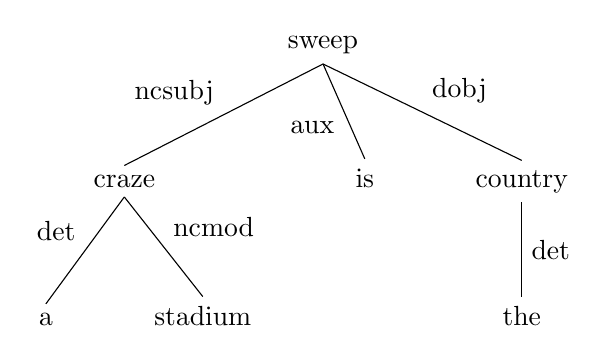
\begin{tikzpicture}[level distance=50pt, sibling distance=30pt]
	      \Tree 
	        [.sweep
	          \edge node[auto=right]{ncsubj}; [.craze  
	            \edge node[auto=right]{det};   [.a ]
	            \edge node[auto=left]{ncmod}; [.stadium ]
	          ]
	          \edge node[auto=right]{aux}; [.is ]
	          \edge node[auto=left]{dobj}; [.country 
	            \edge node[auto=left]{det}; [.the ]
	          ]
	        ]
	    \end{tikzpicture}
		% (ncmod _ craze_2 stadium_1)
		% (det craze_2 A_0)
		% (det country_6 the_5)
		% (dobj sweeping_4 country_6)
		% (aux sweeping_4 is_3)
		% (ncsubj sweeping_4 craze_2 _)
	\end{minipage}
  }
  \subfloat[DRT output from Boxer]{\label{drs:lexical-ambiguity-drs}
    \begin{minipage}[c][0.7\width]{0.5\textwidth}
	  %\centering
		\drs{~x0 x1 e2 x3~}{
		  ~\pred{stadium}{1002}(x0)~ \\
		  ~nn(x0, x1)~ \\
		  ~\pred{craze}{1003}(x1)~ \\
		  ~agent(e2, x1)~ \\
		  ~\pred{sweep}{1005}(e2)~ \\
		  ~event(e2)~ \\
		  ~\pred{country}{1007}(x3)~ \\
		  ~patient(e2, x3)~
		}
	\end{minipage}
  }
  \caption{Dependency parse tree and DRT interpretation of
  sentence \eqref{ex:lexical-ambiguity}}
  \label{drs:lexical-ambiguity}
\end{figure}

The DRS in Figure \ref{drs:lexical-ambiguity-drs}, a formula of logical language
\loglang, shall be denoted by $G$.  Formula $G$ contains a unary predicate
$sweep_{1005}$.  In order to generate weighted substitution rules for
$sweep_{1005}$, we calculate the {\it contextualized inference projection} of
$sweep_{1005}$: the set of inference rules mapping $sweep_{1005}$ to each
(unary) predicate $Q \in \predsym{\loglang}^1$, with each rule weighted by the
similarity of the vector representing the context of $sweep_{1005}$ in $G$ to
the vector representing the replacement $Q$. Since the unary predicate  occurs
in exactly one formula, $G$, we calculate the contextualized inference
projection as
\begin{align*}
&\Pi^G_{\simfunc, \zeta, \ell}(sweep_{1005}) = \\
& \hspace{50px} \{ (F, \eta) \mid \exists Q \in \zeta(P, \predsym{\loglang}^1)~[ \\
& \hspace{110px} F = \forall x.[sweep_{1005}(x) \to Q(x)] \text{ and } \\
& \hspace{110px} \eta = \simfunc\big(\alpha(\ell(sweep_{1005}), \kappa(sweep_{1005}, G)), \ell(Q)\big)~] \}
\end{align*}

Let us assume that our logical language \loglang also includes unary predicates
$cover_{2007}$ and $brush_{3004}$ and that the lemmas {\it cover} and {\it
brush} are known to be synonyms of {\it sweep} (though from different senses). 
In other words, \[ \{ cover_{2007},~ brush_{3004} \} \in \zeta(sweep_{1005},~
\predsym{\loglang}^1) \] So, in the calculation of $\Pi^G_{\simfunc,\zeta
\ell}(sweep_{1005})$, we will generate weighted inference rules $(F,\eta)$ for
both $cover_{2007}$ and $brush_{3004}$.

We look first at $cover_{2007}$.  The rule formula $F$ is instantiated simply as
\[ \forall x.[sweep_{1005}(x) \to cover_{2007}(x)] \]  The weight $\eta$ is the
similarity between the context of $sweep_{1005}$ in $G$, and $cover_{2007}$.
The context vector for $sweep_{1005}$ is calculated as \[
\alpha(\ell(sweep_{1005}), \kappa(sweep_{1005}, G)) \]  Since we defined the
lexical mapping $\ell(P)$ to simply return the vector from $V$ for the lemma
portion of the predicate $P$, $\ell(sweep_{1005}) = \vv{sweep}$ and
$\ell(cover_{2007}) = \vv{cover}$.  

The context of $P$ in $G$, $\kappa(P,G)$ is the set of a set of
predicates and their relations to $P$, so
\begin{align*}
\kappa(sweep_{1005}, G) 
= \{ & (\ell(\pred{stadium}{1002}),~same\text{-}sentence) \} \\
     & (\ell(\pred{craze}{1003}),~same\text{-}sentence), \\ 
     & (\ell(\pred{country}{1007}),~same\text{-}sentence), \\ 
= \{ & (\vv{stadium},~same\text{-}sentence), \\
     & (\vv{craze},~same\text{-}sentence), \\
     & (\vv{country},~same\text{-}sentence) \}
\end{align*}
We defined our contextualization function $\alpha(\vec v, c)$ to be the vector
sum of word vectors from the context $c$, so
\begin{align*}
\alpha(\ell(sweep_{1005}), \kappa(sweep_{1005}, G))
& = \alpha(\vv{sweep},~ \{ 
                (\vv{stadium},~same\text{-}sentence), \\
& \hspace{60px} (\vv{craze},~same\text{-}sentence), \\
& \hspace{60px} (\vv{country},~same\text{-}sentence) \}) \\
& = \vv{stadium} + \vv{craze} + \vv{country}
\end{align*}

Finally, since we have the vector representing the context of $sweep_{1005}$ in
$G$ and the vector representing the replacement predicate $cover_{2007}$, we can
compute the weight, $\eta$ for our inference rule $\forall x.[sweep_{1005}(x)
\to cover_{2007}(x)]$ as
\begin{align*}
& \simfunc\big(\alpha(\ell(sweep_{1005}), \kappa(sweep_{1005}, G)), \ell(Q)\big) \\
& \hspace{120px} = \simfunc\big(\vv{stadium} + \vv{craze} + \vv{country},~ \vv{cover}\big) \\
& \hspace{120px} = cosine\big(\vv{stadium} + \vv{craze} + \vv{country},~ \vv{cover}\big)
\end{align*}
Likewise, the rule for replacing $sweep_{1005}$ by $brush_{3004}$ would be 
$\forall x.[sweep_{1005}(x)$ $\to$ $brush_{3004}(x)]$ weighted by 
$cosine\big(\vv{stadium} + \vv{craze} + \vv{country},~ \vv{brush}\big)$.

Since, $cosine\big(\vv{stadium}$ $+$ $\vv{craze}$ $+$ $\vv{country},~
\vv{cover}\big)$ $>$ $cosine\big(\vv{stadium}$ $+$ $\vv{craze}$ $+$ $\vv{country},~
\vv{brush}\big)$, {\it cover} is considered to be a better replacement for {\it
sweep} than {\it brush} in the sentence ``A stadium craze is sweeping the
country''.  Thus, the rule $\forall x.[sweep_{1005}(x) \to cover_{2007}(x)]$
will be given more consideration during inference.


% \subsection*{Hypernymy}
% 
% \entpairex{ex:hyp-0}{Ed owns a car.}{Ed has a automobile.}
% 	
% Even restricting rules to wordnet relationships, \eqref{ex:hyp-0} works in
% because car and automobile are synonyms (in the same synset).
% We construct rule 
% 
% $(w,~ car \to automobile)$ where w = $sim(ctx(car),~ automobile)$
% 
% \entpairex{ex:hyp-1}{Ed owns a car.}{Ed has a vehicle.}
% 
% Even restricting rules to wordnet relationships, this works because vehicle
% is a hypernym of (a sense of) car.
% We can construct a rule 
% 
% $(w,~ car \to vehicle)$ where w = $sim(ctx(car),~ vehicle)$
% 
% \entpairex{ex:hyp-2}{Ed owns a vehicle.}{Ed has a car.}
% 
% This is a less likely, but not altogether terrible entailment.
% However, using wordnet strictly would fail since vehicle is a hypernym of (a
% sense of) car.
% So, instead of strictly limiting our rules to wordnet relationships, we could
% have separate rules with separate weights:
% 
% $(w_1,~ vehicle \to car)$ where $w_1 = sim(ctx(vehicle), car)$ 
% 
% $(w_2,~ vehicle \to \lnot car)$ where $w_2$ = a measure of how far {\it car} and
% {\it vehicle} are in the hierarchy.
% 
% So, we can say that, with certainty w1, that 'car' fits into 'vehicle''s context
% based on distributional data.
% Further, we can say with certainly w2 that 'vehicle' can be replaced with 'car'
% based on ontology data.
% 
% 
% 
% \subsection*{Integration between logical and distributional phenomena}
% 
% 
% 
% Some natural language phenomena are most naturally treated as categorial, while
% others are more naturally treated using weights or probabilities. In this paper,
% we treat implicativity, while using a probabilistic approach to word meaning.
% 
% 
% 
% For example \eqref{ex:ws-imp-1}, ``fail to'' is a negatively entailing
% implicative in a positive environment.
% So, $p$ correctly entails $h_{good}$ in both the theorem prover and Alchemy. 
% However, the theorem prover incorrectly licenses the entailment of $h_{bad}$
% while Alchemy does not.  
% The probabilistic approach performs better in this situation because the
% categorial approach does not distinguish between a good paraphrase and a
% bad one.  This example also demonstrates the advantage of using a
% context-sensitive distributional model to calculate the probabilities of
% paraphrases because ``reward'' is an {\it a priori} better paraphrase than
% ``observe'' according to WordNet since it appears in a higher ranked synset. 
% 
% \begin{covex}\label{ex:ws-imp-1}
% \begin{itemize}
%   \item[$p$:] The U.S. is watching closely as South Korea fails to honor
%   U.S. patents\footnote{Example \eqref{ex:ws-imp-1} is adapted from Penn
%   Treebank document wsj\_0020 while \eqref{ex:ws-imp-2} is adapted from document
%   wsj\_2358}
%   \item[$h_{good}$:] South Korea does not {\bf observe} U.S. patents
%   \item[$h_{bad}$:] South Korea does not {\bf reward} U.S. patents
% \end{itemize}
% \end{covex}
% 
% 
% 
% 
% Above, we stated that the entailment in \eqref{ex:hyp-1} was licensed because a
% {\it car} is a type of {\it vehicle} and we can entail from a subset to a
% superset.  In fact, the situation is complicated a bit because the direction of
% entailment is actually dictated by the polarity of the context in which the
% words appear.
% 
% Consider example \eqref{ex:hyp-3} below
% \entpairex{ex:hyp-3}{Ed does not own a vehicle.}{Ed does not have a car.}
% This entailment is valid despite the fact that we are entailing from {\it
% vehicle} to {\it car}, the opposite direction as in example \eqref{ex:hyp-1}. 
% The difference is that in \eqref{ex:hyp-1}, the words appeared in a {\it
% positive context} while in \eqref{ex:hyp-3} they appear in a {\it
% negative context} since they are embedded under a single negation.
% 
% However, the approach that we have chosen to take handles this interaction
% naturally.  The softened inference rules we generate for hypernym relationships
% may lower the probability of entailment versus a similar hard rule (when the
% weight is less than 1), but if an entailment rule does not fit the polarity of
% the context, then it will not raise the probability of entailment.
% 
% In addition to negation, other linguistic constructs such as quantifiers and
% implicative verbs may affect the polarity of a context
% \citep{maccartney:iwcs2009}.  Our system handles all equally well.
% 

\section{Implicatives and factives}

[TODO: It would be nice if this also fit into the interface framework\ldots]

\citet{nairn:icos2006} presented an approach to the treatment of inferences
involving implicatives and factives.  Their approach identifies an ``implication
signature'' for every implicative or factive verb that determines the truth
conditions for the verb's nested proposition, whether in a positive or negative
environment.  Implication signatures take the form ``$x/y$'' where $x$
represents the implicativity in the the positive environment and $y$ represents
the implicativity in the negative environment.  Both $x$ and $y$ have three
possible values: ``+'' for positive entailment, meaning the nested proposition
is entailed, ``-'' for negative entailment, meaning the negation of the proposition
is entailed, and ``o'' for ``null'' entailment, meaning that neither the
proposition nor its negation is entailed. Figure \ref{fig:imp-sig} gives
concrete examples.% for two signatures.

% For example, the verb ``managed to'' has positive entailment in the {\it true}
% case and negative entailment under negation.  So, {\it he managed to escape
% $\vDash$ he escaped} while {\it he did not manage to escape $\vDash$ he did not
% escape}.  On the other hand, the verb ``refused to'' has negative entailment
% in the positive case and ``null'' entailment under negation.  So, {\it he
% refused to fight $\vDash$ he did not fight} but {\it he did not refuse to fight}
% entails neither {\it he fought} nor {\it he did not fight}.

\begin{figure}
\begin{center}
  \begin{tabular}{l c l}
    \hline
   	 & ~~~~~~signature~~~~~~ &  \multicolumn{1}{c}{example} \\
   	\hline
%    	admitted that    & +/+ & he admitted that he knew $\vDash$ he knew \\
%    	                 &     & he did not admit that he knew $\vDash$ he knew \\
%    	\hline
   	forgot that      & +/+ & he forgot that Dave left $\vDash$ Dave left \\
   	                 &     & he did not forget that Dave left $\vDash$ Dave left \\
   	\hline
%    	pretended that   & -/- & he pretended he was sick $\vDash$ he was not sick \\
%    	                 &     & he did not pretend he was sick $\vDash$ he was not sick\\
%    	\hline
%    	wanted to        & o/o & he wanted to fly $?$ he flew \\  
%    	                 &     & he did not want to fly $?$ he flew \\
%    	\hline
   	managed to       & +/- & he managed to escape $\vDash$ he escaped \\
   	                 &     & he did not manage to escape $\vDash$ he did not escape \\
   	\hline
%    	was forced to    & +/o & he was forced to sell $\vDash$ he sold \\
%    	                 &     & he was not forced to sell $?$ he sold \\
%    	\hline
%    	was permitted to & o/- & he was permitted to leave $?$ he left \\
%    	                 &     & he was not permitted to leave $\vDash$ he did not leave \\
%    	\hline
   	forgot to        & -/+ & he forgot to pay $\vDash$ he did not pay \\
   	                 &     & he did not forget to pay $\vDash$ he paid \\
   	\hline
   	refused to       & -/o & he refused to fight $\vDash$ he did not fight \\
   	                 &     & he did not refuse to fight $\nvDash$ \{he fought, he did not fight\} \\
   	\hline
%    	hesitated to     & o/+ & he hesitated to ask $?$ he asked\\
%    	                 &     & he did not hesitate to ask $\vDash$ he asked \\
%    	\hline
  \end{tabular}
\end{center}
\caption{Implication Signatures}
\label{fig:imp-sig}
\end{figure}


\subsection*{Inferences with nested propositions}

The standard conversion from DRT to first-order logic (FOL) (the one used by
Boxer), falls short on nested propositions.  Consider the entailment pair ``John
did not manage to leave'' and ``John left''.  The DRT interpretation and its
corresponding FOL conversion are are shown in Figure \ref{drs:impl-1}.

\begin{figure}
  \centering
  \subfloat[DRT interpretation]{\label{drs:impl-1-drt}
    ~~~~~~~~
	\drs{~x0~}{
	  ~john_{1001}(x0)~ \\
	  \negdrs{~e1 p2~}{
	    ~manage_{1004}(e1)~ \\
	    ~agent(e1, x0)~ \\
	    ~theme(e1, p2)~ \\
	    ~p2:~\drs{~e3~}{
	      ~leave_{1006}(e3)~ \\
	      ~agent(e3, x0)~
	    }
	  }
	}
	~~~~~~~~
  }
  ~~~~~~~~~
  \subfloat[FOL translation]{\label{drs:impl-1-fol}
    \dhgboxed{$
      ~\exists~ x0.[
      ~  john_{1001}(x0) ~\&~ \\
      ~  \hspace{18px} \lnot \exists~ e1 p2.[
      ~                  manage_{1004}(e1) ~\&~ \\
      ~    \hspace{55px} agent(e1, x0) ~\&~ \\
      ~    \hspace{55px} theme(e1, p2) ~\&~ \\
      ~    \hspace{55px} \exists~ e3.[
      ~                    leave_{1006}(e3) ~\&~ \\
      ~      \hspace{77px} agent(e3, x0) ]]]
    $}
%     ~~~~~~~~
% 	\drs{~x0 e1~}{
% 	  ~john_{2001}(x0)~ \\
% 	  ~leave_{2002}(e1)~ \\
% 	  ~agent(e1, x0)~
% 	}
% 	~~~~~~~~
  }
  \caption{Boxer's DRT interpretation of ``John did not manage to leave.''.}
  \label{drs:impl-1}
\end{figure}

While it should be clear that ``John did not manage to leave'' does {\it not}
entail ``John left'' (and, in fact, entails the opposite), the FOL formula shown
in Figure \ref{drs:impl-1-fol} {\it does} entail the FOL representation of
``John left'' \[ \exists~ x0~e1.[john_{1001}(x0) ~\&~ leave_{1006}(e1) ~\&~
agent(e1, x0)] \]  

The incorrect inference occurs here because the standard DRT-to-FOL translation
loses some information.  DRT expressions are allowed to have {\it labeled
subexpressions}, such as $p2$ in Figure \ref{drs:impl-1-drt} that is used to
reference the {\theme} of the {\it manage} event: the {\it leave} event.  The
FOL expression, on the other hand, shows that $p2$ is the theme of event $e1$,
but has no way of stating what $p2$ refers to.

In order to capture the information that the DRT labels provide, we modify the
DRT expression to contain explicit {\it subexpression triggers}.  That is, for a
sub-DRS $A$ labeled by $p$, we replace $A$ with two new expressions in the same
scope: $POS(p) \to A$ and $NEG(p) \to \lnot A$.  The result of such a
replacement on the DRS in \ref{drs:impl-1-drt} can be see in Figure
\ref{drs:impl-2-drt}.   

\begin{figure}
  \centering
  \subfloat[DRT interpretation with subexpression triggers]{\label{drs:impl-2-drt}
	\drs{~x0~}{
	  ~john_{1001}(x0)~ \\
	  ~\drs{~p2~}{
	    ~\negdrs{~e1~}{
	      ~manage_{1004}(e1)~ \\
	      ~theme(e1, p2)~ \\
	      ~agent(e1, x0)~} \\
	    \unboxedifdrs{POS(p2)}{   \drs{~e3~}{~leave_{1006}(e3)~ \\ ~agent(e3, x0)~}} \\
	    \unboxedifdrs{NEG(p2)}{\negdrs{~e3~}{~leave_{1006}(e3)~ \\ ~agent(e3, x0)~}}
	  }
	}
  }
  ~~~~~~~~~
  \subfloat[Subexpression-triggering inference rules for implicative ``manage
            to'' with signature +/-]{\label{drs:impl-2-rules} 
  \shortstack{
      \unboxedifdrs{\drs{~p~}{~   \drs{~e~}{~manage_{1004}(e)~ \\ ~theme(e, p)~}~}}{POS(p)} \\
      \\\\\\\\\\\\
      \unboxedifdrs{\drs{~p~}{~\negdrs{~e~}{~manage_{1004}(e)~ \\ ~theme(e, p)~}~}}{NEG(p)}
    }
  }
  \caption{First (insufficient) attempt at correcting for the loss of labeled
  sub-expression information.}
  \label{drs:impl-2}
\end{figure}

Now that our labeled subexpression has triggers, we can introduce inference
rules to activate those triggers.  The purpose of these inference rules is to
capture the behavior dictated by the implication signature of the implicative
verb for which the relevant subexpression is the theme.  For example, according
to the implication signature, the implicative {\it manage to} is positively
entailing in positive contexts and negatively entailing in negative contexts.
This means that if John {\it managed to} do what is described by $p$, then the
event described by $p$ occurred, or in other words, the subexpression of $p$ is
{\it true}. Likewise, if John {\it did not manage to} do what is described by
$p$, then the event described by $p$ {\it did not} occur, meaning that the
subexpression of $p$ is {\it false}.  

The triggering inference rules for {\it managed to} are shown in Figure
\ref{drs:impl-2-rules}.  The first rule, for positive contexts, says that for
all propositions $p$, if $p$ is ``managed'', then $p$'s subexpression is {\it
true}, so trigger the ``positive entailment'' subexpression which, in our
example, says that the {\it leaving} event occurred.  The second rule, for
negative contexts, says that for all propositions $p$, if there is {\it no}
``managing'' of $p$, then $p$'s subexpression is {\it false}, so trigger the
``negative entailment'' subexpression to say that there is {\it no} event of
{\it leaving}.

While this approach works for positive contexts, there is a subtle problem for
negative contexts.  The negative context rule in Figure \ref{drs:impl-2-rules}
can be translated to FOL as \[ \forall~ p.[~ \lnot \exists~ e.[~ manage(e) \land
theme(e,p)) ~] \to NEG(p) ~] \] This expression is stating that for all
propositions $p$, $p$ is {\it false} if there is no ``managing'' of $p$.  Now,
we want this inference rule to be used in cases where it is stated that
``managing'' did not occur, such as in the expression of Figure
\ref{drs:impl-2-drt}, where we see that is is the case that \[ ~\negdrs{~x0 e1
p2~}{ ~manage_{1004}(e1)~ \\ ~agent(e1, x0)~ \\ ~theme(e1, p2)~} \] which is
equivalent to the FOL expression \[ \lnot manage_{1004}(e1) \land \lnot
agent(e1, x0) \land \lnot theme(e1, p2) \] stating that $e1$ is a ``managing''
of $p2$ by $x0$.  However, the antecedent of our negative context rule states
that there is {\it no} ``managing'' of the proposition, so the rule would only
be used if it could be proven that there is no ``managing'' at all.
Unfortunately, stating that $p2$ is not ``managed'' {\it by x0} does {\it not}
entail that $p2$ is not ``managed'' at all since $p2$ could be managed by
someone other than $x0$.

To overcome this problem, we modify our representation of a negated event. 
Instead of representing an event, such as the ``managing'' event, that that
{\it did not} occur as $\lnot \exists~ e.[~ manage(e) ~]$, we represent it
explicitly as an event of {\it non-occurrence}: $\exists~ e.[~
\textbf{not\_}manage(e) ~]$.  Applying this change to the DRS and inference
rules in Figure \ref{drs:impl-2}, we arrive at our final form in Figure
\ref{drs:impl-3}.

\begin{figure}
  \centering
  \subfloat[DRT interpretation with subexpression triggers]{\label{drs:impl-3-drt}
	\drs{~x0~}{
	  ~john_{1001}(x0)~ \\
	  ~\drs{~e1 p2~}{
	    ~\textbf{not\_}manage_{1004}(e1)~ \\
	    ~theme(e1, p2)~ \\
	    \negdrs{ }{~agent(e1, x0)~} \\
	    \unboxedifdrs{POS(p2)}{\drs{~e3~}{~              leave_{1006}(e3)~ \\ ~agent(e3, x0)~}} \\
	    \unboxedifdrs{NEG(p2)}{\drs{~e3~}{~\textbf{not\_}leave_{1006}(e3)~ \\ \negdrs{ }{~agent(e3, x0)~}}}
	  }
	}
  }
  ~~~~~~~~~
  \subfloat[Subexpression-triggering inference rules for implicative ``manage
            to'' with signature +/-]{\label{drs:impl-3-rules} 
  \shortstack{
      \unboxedifdrs{\drs{~p~}{~\drs{~e~}{~              manage_{1004}(e)~ \\ ~theme(e, p)~}~}}{POS(p)} \\
      \\\\\\\\\\\\
      \unboxedifdrs{\drs{~p~}{~\drs{~e~}{~\textbf{not\_}manage_{1004}(e)~ \\ ~theme(e, p)~}~}}{NEG(p)}
    }
  }
  \caption{Explicit capturing of sub-expression information.}
  \label{drs:impl-3}
\end{figure}

Using this strategy, we can see that the negative context rule is active when
there exists a ``not-managing'' event, and the representation of ``John did
not manage to leave'' explicitly states that there is such an event, meaning
that the rule will be used in the inference.  With all of these pieces in place,
the inference works as expected.

Thus, we transform the output of Boxer in two ways.  First, we identify any
labeled propositions and replace them with pairs of proposition triggers.  Then,
we modify any negated DRSs by extracting the verb and theme atoms, changing the
verb predicate to a ``not\_'' predicate, and finally ensuring that all other
expressions under the negated DRS (aside from the labeled proposition itself),
remain under a negated DRS.

Once the sentence representations have been modified, we generate inference
rules for each implicative verb.  If the verb is positively entailing in
positive contexts, we generate a rule of the form 
\[ \forall~ p.[~ \exists~ e.[~ \langle verb \rangle(e) \land theme(e,p)) ~] \to POS(p) ~] \]
but if it is negatively entailing in positive contexts, we instead generate a rule of the form
\[ \forall~ p.[~ \exists~ e.[~ \langle verb \rangle(e) \land theme(e,p)) ~] \to NEG(p) ~] \]
If the verb is positively entailing in {\it negative} contexts, we generate a rule of the form
\[ \forall~ p.[~ \exists~ e.[~ \textbf{not\_}\langle verb \rangle(e) \land theme(e,p)) ~] \to POS(p) ~] \]
but if it is negatively entailing in negative contexts, we instead generate a rule of the form
\[ \forall~ p.[~ \exists~ e.[~ \textbf{not\_}\langle verb \rangle(e) \land theme(e,p)) ~] \to NEG(p) ~] \]
If the verb is non-entailing in either positive or negative contexts, then we do
not generate a rule for that context polarity. 

This approach works for arbitrarily long chains of nested implicatives.  It also
interacts properly with 



\subsection*{Use of subcategorization frame}

The the verb {\it forget} has different implicative properties depending on its
subcategorization frame.  When used as {\it forget that}, as in ``He forgot that
Dave left'', it is positively entailing in both positive and negative contexts. 
When used as {\it forget to}, as in ``He forgot to lock the door'', it is
negatively entailing in positive contexts and positively entailing in negative
contexts.

In order to generate the correct inference rules, the right implication
signature must be selected.  To do this, we make use of the dependency parse
generated by the C\&C parser that is input to Boxer.  The parse tells us which
version of the verb is being used.  In our example ``He forgot that
Dave left'', {\it forgot} has a ``ccomp'' relationship to the {\it left}, while
in ``He forgot to lock the door'', {\it forgot} has a ``xcomp+to'' relationship
to {\it lock}.



\subsection*{Weighting implicative inference rules}

While we do not have a scheme for generate such weights at this time, one of the
advantages of our approach is that it allows for the independent weighting of
each implicative inference rule in isolation.  


\section{Evaluation and phenomena}

Textual entailment offers a good framework for testing whether a
system performs correct analyses and thus draws the right inferences
from a given text. For example, to test whether a system correctly
handles implicative verbs, one can use the \emph{premise} $p$ along with
the \emph{hypothesis} $h$ in \eqref{ex:imp-fact-nested} below. If the system
analyses the two sentences correctly, it should infer that $h$ holds.
While the most prominent forum using textual entailment is the 
Recognizing Textual Entailment (RTE) challenge \citep{dagan:rte2005},
the RTE datasets 
do not test the phenomena in which we are interested.
For example, in order to evaluate our system's ability to determine word meaning
in context, the RTE pair would have to specifically test word sense confusion by
having a word's context in the hypothesis be different from the context of the
premise.  However, this simply does not occur in the RTE corpora.  In order to
properly test our phenomena, we construct hand-tailored premises and hypotheses
based on real-world texts.


In this paper, we focus on three natural language phenomena and their
interaction: implicativity and factivity, word meaning, and coreference.
The first phenomenon, implicativity and factivity, is concerned with analyzing
the truth conditions of nested propositions.  For example, in the premise of
the entailment pair shown in example 
\eqref{ex:imp-fact-nested}, ``arrange that'' falls under the scope of 
``forget to'' and ``fail'' is under the scope of ``arrange that''.
Correctly recognizing nested propositions is necessary for preventing
false inferences such as the one
in example \eqref{ex:hope-build}.

\begin{example}\label{ex:imp-fact-nested}
\begin{itemize}
  \item[$p$:] Ed did not forget to arrange that Dave 
fail\footnote{Examples \eqref{ex:imp-fact-nested}
and \eqref{ex:imp-fact-hyper} and Figure \ref{fig:imp-sig} are based on examples by
\citet{maccartney:iwcs2009}}
  \item[$h$:] Dave failed
\end{itemize}
\end{example}

\begin{example}\label{ex:hope-build}
\begin{itemize}
  \item[$p$:] The mayor hoped to build a new stadium\footnote{Examples
\eqref{ex:hope-build}, \eqref{ex:prob-wordsense}, \eqref{ex:coref}, and
\eqref{ex:ws-coref} are modified versions of sentences from document wsj\_0126
from the Penn Treebank}
  \item[$h$*:] The mayor built a new stadium
\end{itemize}
\end{example}


For the second phenomenon, word meaning, we address paraphrasing and
hypernymy.  For example, in \eqref{ex:prob-wordsense} ``covering'' is a good
paraphrase for ``sweeping'' while ``brushing'' is not.

\begin{example}\label{ex:prob-wordsense}
\begin{itemize}
  \item[$p$:]   A stadium craze is \textbf{sweeping} the country
  \item[$h_1$:] A stadium craze is \textbf{covering} the country
  \item[$h_2$*:] A stadium craze is \textbf{brushing} the country
\end{itemize}
\end{example}

The third phenomenon is coreference, as illustrated in \eqref{ex:coref}.  For
this example, to correctly judge the hypothesis as entailed, it is necessary
to recognize that ``he'' corefers with ``Christopher'' and ``the new ballpark''
corefers with ``a replacement for Candlestick Park''.

\begin{example}\label{ex:coref}
\begin{itemize}
  \item[$p$:] George Christopher has been a critic of the plan to build a
  replacement for Candlestick Park. As a result, he won't endorse the new ballpark.
  \item[$h$:] Christopher won't endorse a replacement for Candlestick Park.
\end{itemize}
\end{example}

Some natural language phenomena are most naturally treated as categorial, while 
others are more naturally treated using weights or 
probabilities. In this paper, we treat implicativity and coreference
as categorial phenomena, while using a probabilistic approach to word
meaning. 


\section{Preliminary Evaluation}

As a preliminary evaluation of our system, we constructed the set of 
demonstrative examples included in this paper to test our system's ability
to handle the previously discussed phenomena and their interactions.  We ran
each example with both a standard first-order theorem prover and Alchemy to
ensure that the examples work as expected. Note that since weights are not
possible when running an example in the theorem prover, any rule that would 
receive a non-zero weight in an MLN is simply treated as a ``hard clause'' following
\citet{bos:emnlp2005}.  For the experiments, we generated a vector space from
the entire New York Times portion of the English Gigaword corpus
\citep{graff:gigaword2003}.

The example entailments evaluated were designed to test the interaction between
the logical and weighted phenomena.  For example, in \eqref{ex:ws-imp-1}, ``fail
to'' is a negatively entailing implicative in a positive environment, so according 
to the theorem prover, $p$ entails both {\it h1} and {\it h2}.  However, using our
weighted approach, Alchemy outputs that {\it h1} is more probable than {\it h2}. 
\begin{covex}\label{ex:ws-imp-1}
\begin{itemize}
  \item[{\it p:}]~~    The U.S. is watching closely as South Korea fails to honor
  U.S. patents\footnote{Sentence adapted from Penn Treebank document wsj\_0020.}
  \item[{\it h1:}]~~~~South Korea does not {\bf observe} U.S. patents
  \item[{\it h2*:}]~~~~South Korea does not {\bf reward} U.S. patents
\end{itemize}
\end{covex}
The first-order approach, which contains inference rules for both
paraphrases as hard clauses, cannot distinguish between
good and bad paraphrases, and considers both of them equally valid. In
contrast, the weighted approach can judge the degree of fit of the two potential
paraphrases. Also, it does so in a context-specific manner, choosing
the paraphrase {\it observe} over {\it reward} in the context of
{\it patents}. 

Our ability to perform a full-scale evaluation is currently limited by problems
in the Alchemy software required to perform probabilistic inference.  This is
discussed more in Section \ref{sec:future}.

\section{Future work}

Or plans for continued word can be divided into two categories: word on the
theoretical side and work on implementation.

From a theoretical perspective, we have used a simplistic bag-of-words
approach for
computing a context-specific vector for a predicate based on its
formula context. We plan to move to a more informative construction
that takes semantic relations into account. This will be interesting in particular because the relations that can be read off a logical
form differ from those available in a dependency parse. For example,
we can check whether two predicates occur within the same DRS, or
whether they apply to a common variable. We can also ask what 
influence different logical connectives have on perceived word meaning. 


We would also like to extend our formalism to address
a wider range of linguistic phenomena.  Many phenomena are better
described using weights than through categorial analyses, and first-order representations do not correctly
address this.  By extending our framework, we hope to be able to
apply weights derived from distributional information to a wide variety of
modeled concepts.


% [think about vector spaces that take logical form into account similar to how
% pado and lapata took dependencies into account.]

From an implementation perspective, we would like to %produce a dataset that
%tests all of the issues outlined in this paper, and to 
run a large-scale
evaluation of our techniques.  
However, the major barrier here is that the Alchemy software has severe
inefficiencies in terms of memory requirements and speed, preventing us
from executing larger and more complex examples.  There is on-going
work to improve Alchemy [TODO: CITE Vibhav's PTP paper].

% KE: let's not go there yet. This would take too much time to explain.
% We are also interested in comparing our approaches to recent work on building
% vectors from entire sentences [TODO: CITATIONS].  We would like to example
% how our approach compares in the task of measuring similarity between
% phrases.


\section{Conclusion}

In this paper, we have defined a link between logical form and vector
spaces through a lexical mapping of predicate symbols to points in
space. We address polysemy not through separate predicate symbols for
different senses of a word, but by using a single predicate symbol
with a lexical mapping that gets
adapted to the context in which the predicate symbol appears. We use
the link to project weighted inferences from the vector space to the
logical form. 

We showed how these weighted first-order
representations can be used to perform probabilistic first-order inferences
using Markov Logic.  We have shown how our approach handles three distinct
phenomena, word meaning ambiguity, hypernymy, and implicativity, as well as
allowing them to interact appropriately.  Most importantly our approach allows 
us to model some phenomena with hard first-order techniques and
others phenomena with soft weights, and to do all of them within a
single, unified framework.
The resulting approach is able to correctly solve a number of difficult
textual entailment problems that require handling complex combinations of these
important semantic phenomena.

% The framework we have developed takes a pair of natural
% language sentences as input and parses them into DRS \citep{kamp:book93}
% representations.  It then augments those representations by linking the
% predicates back to the original words in the sentences and incorporating
% coreference information from OntoNotes \citep{hovy:naacl2006}.
% Since DRSs are hierarchical structures, our approach flattens them to a simple
% list of atoms while keeping track of the original structure through DRS labels
% as arguments, allowing inferences to be performed in 
% an MLN. In order to maintain the DRS semantics in the flat logical form, we have 
% hand-written a collection of inference rules that are used in the inference. 
% We also generate a list of inference rules to address the particular
% linguistic phenomena that we are handling.  Categorial rules based
% on implication signatures \citep{nairn:icos2006} are used to handle
% implicativity and factivity.  Weighted rules are used to address issues of
% word meaning in context.



\section*{Acknowledgements}

This work was supported by the Department of Defense (DoD) through a
National Defense Science and Engineering Graduate Fellowship (NDSEG) Fellowship
for the first author, National Science Foundation grant IIS-0845925 for the
second author, and a grant from the Longhorn Innovation Fund for Technology.
[TODO: Is all of this right?]




\bibliographystyle{styles/spbasic}
\bibliography{mln-sem}

\end{document}

